\documentclass[10pt,landscape]{article}
\usepackage{multicol}
\usepackage{multirow}
\usepackage{calc}
\usepackage{ifthen}
\usepackage[landscape]{geometry}
\usepackage{hyperref}
\usepackage{graphicx}
\usepackage[export]{adjustbox}
\usepackage{subcaption}
\usepackage{wrapfig}

\geometry{top=1cm,left=1cm,right=1cm,bottom=1cm} 

% Turn off header and footer
\pagestyle{empty}

% Redefine section commands to use less space
\makeatletter
\renewcommand{\section}{\@startsection{section}{1}{0mm}%
                                {-1ex plus -.5ex minus -.2ex}%
                                {0.5ex plus .2ex}%x
                                {\normalfont\large\bfseries}}
\renewcommand{\subsection}{\@startsection{subsection}{2}{0mm}%
                                {-1explus -.5ex minus -.2ex}%
                                {0.5ex plus .2ex}%
                                {\normalfont\normalsize\bfseries}}
\renewcommand{\subsubsection}{\@startsection{subsubsection}{3}{0mm}%
                                {-1ex plus -.5ex minus -.2ex}%
                                {1ex plus .2ex}%
                                {\normalfont\small\bfseries}}
                                
\newcommand*\dotcolumnfill{
    \par
    \null
    \vskip -\ht\strutbox
    \xleaders \hb@xt@ \hsize {
        \strut \cleaders \hb@xt@ .44em{\hss.\hss}\hfill
    }\vfill
    \vskip \ht\strutbox
    \break
}
\makeatother

% Define BibTeX command
\def\BibTeX{{\rm B\kern-.05em{\sc i\kern-.025em b}\kern-.08em
    T\kern-.1667em\lower.7ex\hbox{E}\kern-.125emX}}

% Don't print section numbers
\setcounter{secnumdepth}{0}

\setlength{\parindent}{0pt}
\setlength{\parskip}{0pt plus 0.5ex}


% -----------------------------------------------------------------------

\begin{document}

\raggedright
\footnotesize

\begin{center}
     \Large{\textbf{Recordatorio: Open Water}} \\
\end{center}

\begin{multicols*}{3}

% multicol parameters
\setlength{\premulticols}{1pt}
\setlength{\postmulticols}{1pt}
\setlength{\multicolsep}{1pt}
\setlength{\columnsep}{2pt}

\section{Siempre}
\begin{itemize}
\item {\bfseries Lleva un compañero}
\item {\bfseries Respira continuamente} y nunca dejes de respirar (incluso exhala de forma continua cuando no tengas el regulador en la boca)
\item Respira lenta y profundamente
\item Si tienes un problema, para y recupera la respiración lenta y profunda antes de continuar
\end{itemize}

\section{Señas}

\begin{center}
\includegraphics[width=\columnwidth]{señas.png}
\end{center}

\section{Antes de la inmersión}

Planea una inmersión que no sobrepase tu experiencia y te haga sentir cómodo.
Intenta no llegar cansado, empachado, ni de resaca.  Cancela la inmersión si notas que estás enfermo (especialmente si tienes los oidos o fosas nasales taponadas). \\
Comprueba las predicciones (\texttt{tablademareas.com}).  Al planear la inmersión, ten en cuenta que el perfil ideal sería empezar en el punto más profundo e ir subiendo lentamente.
\columnbreak

\section{Equipo Autónomo}
\subsubsection{Regulador}

Proporciona aire a la presión del entorno cuando inhalas y expulsa al agua el aire exhalado.

\begin{center}
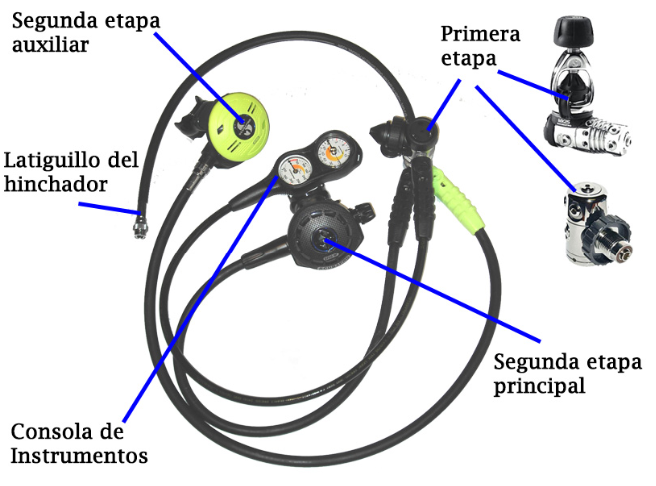
\includegraphics[width=\columnwidth]{regulador.png}
\end{center}

\subsubsection{Chaleco, jacket o BCD}
A él va enganchado el resto del equipo y te permite ajustar la flotabilidad durante la inmersión.

\begin{center}
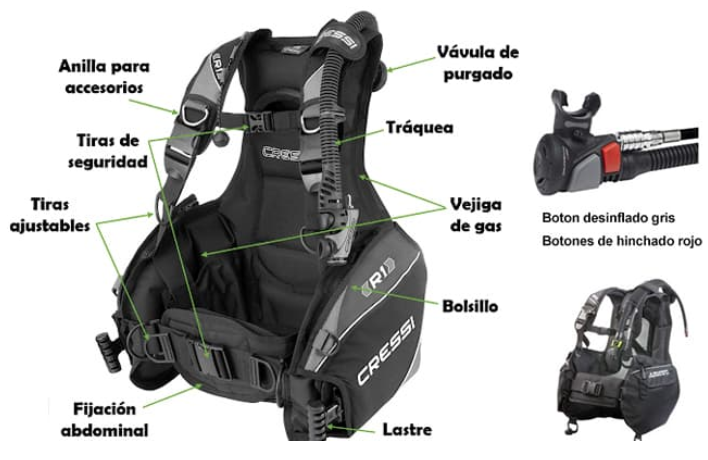
\includegraphics[width=\columnwidth]{bcd.png}
\end{center}
\columnbreak

\subsection{Preparación del equipo}

Comprueba el equipo. No bucees con ningún elemento del equipo que no esté en buenas condiciones.\\
Usa la cantidad de lastre adecuada, para poder controlar bien tu flotabilidad.\\
Prepara el equipo:
\begin{enumerate}
\item Desplaza el chaleco por la botella con la apertura de la grifería mirando hacia el chaleco. Ajusta las tiras para que sujeten la botella. A continuación, levanta el chaleco para asegurarte de que la botella no se desliza.
\begin{center}
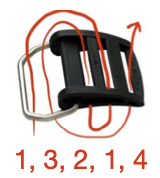
\includegraphics[width=0.3\columnwidth]{enganche_botella.png}
\centerline{\textit{Cómo enganchar las tiras del chaleco}}
\centerline{\textit{para que sujeten bien la botella}}
\end{center}

\item Asegúrate de que la junta tórica no está dañada o sucia, enrosca la primera etapa en la apertura de la grifería de forma que el latiguillo del hinchador vaya hacia el lado de la tráquea.
\item Conecta el latiguillo con el chaleco.
\item Gira la consola de instrumentos lejos de ti y abre la botella. Comprueba que el aire se mantiene y hay suficiente para la inmersión.
\end{enumerate}
También comprueba:
\begin{itemize}
\item Botones de purga (el aire debe parar al soltar)
\item Respirar por la segunda etapa principal y auxiliar
\item Hinchado y desinflado del chaleco
\end{itemize}
Si no lo vas a usar un rato, cierra la botella y purga el aire del chaleco.
Ajusta tu chaleco hasta que te quede ceñido. Después, hínchalo por completo para garantizar que no restringe tu respiración.

\section{Tamaños del Equipo}
\begin{center}
\renewcommand{\arraystretch}{1.2}
\begin{tabular}{|p{0.2\columnwidth}|p{0.7\columnwidth}|} 
\hline
Escarpines &  \\ 
\hline
Neopreno &  \\ 
\hline
Chaleco &  \\ 
\hline
\end{tabular}
\end{center}
\columnbreak

\section{En el barco}
Asegurate de que tanto tú como tu compañero teneis los trajes bien ajustados y el chaleco completamente hinchado antes de entrar en el agua.

\begin{center}
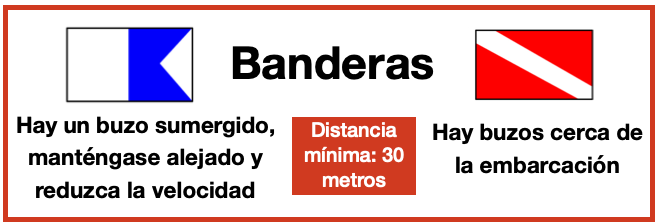
\includegraphics[width=\columnwidth]{banderas.png}
\end{center}


\section{Descendiendo}

\textbf{Contrarresta el aumento de presión de aire.}\\
Compensa cada metro, antes de sentir molestias.\\
Para compensar los oídos y senos nasales, tápate la nariz y sopla suavemente por ella (nunca con fuerza). A algunas personas también les funciona mover la mandíbula de lado a lado o tragar saliva.\\
Para compensar la máscara, añádele aire soplando por la nariz.\\
Si no consigues compensar, asciende ligeramente hasta que se te pase la molestia y vuelve a intentarlo. Ten paciencia. Si no lo consigues, interrumpe la sesión.\\ 
\textbf{Corrige la flotabilidad:} Al bajar la densidad del aire aumenta, añade aire al chaleco para mantener una flotabilidad neutra.

\section{Durante la inmersión}
\begin{itemize}
\item  \textbf{Temperatura:} Se transmite más rápido. Cuidado con el frío.
\item  \textbf{Luz:} Se vuelve más oscuro. Los colores se van perdiendo, los rojizos primero.
\item  \textbf{Sonidos:} Viajan más lejos y 4 veces más rápido. Es difícil determinar su origen.
\end{itemize}

\begin{center}
\renewcommand{\arraystretch}{1.2}
\begin{tabular}{ |c|c|c|c| } 
\hline
\multirow{2}{0.2\columnwidth}{Profundidad (metros)} & \multirow{2}{0.2\columnwidth}{Presión (bar)} & \multirow{2}{0.2\columnwidth}{Volumen de aire} & \multirow{2}{0.2\columnwidth}{Densidad de aire} \\
 &  & & \\ 
 \hline
 \hline
0 & 1 & 1 & x1 \\ 
 \hline
10 & 2 & 1/2 & x2 \\ 
 \hline
20 & 3 & 1/3 & x4 \\ 
\hline
\end{tabular}
\end{center}

\textbf{Respira lento y profundo.}\\
Se usa más aire con más:
\begin{itemize}
\item \textbf{Profundidad:} sigue la misma relación que el volumen de aire (p.e. 1/2 de tiempo a 10 metros)
\item \textbf{Velocidad de respiración:} Intenta moverte lo mínimo, relajarte y mantener un ritmo respiratorio constante. El doble de rápido supone 4 veces más gasto
\end{itemize}
Usa el chaleco para mantener una flotabilidad neutra. Para hinchar el chaleco con la boca, pulsa el botón de desinflado mientras soplas.


\section{Ascendiendo}

\textbf{Respira de forma continua.}\\
Si sientes molestias al ascender (bloqueo inverso), baja un par de metros, esperar un poco y asciende a menor velocidad.\\
\textbf{Corrige la flotabilidad:} Al ascender, la densidad de aire se reduce, quita aire al chaleco para mantener una flotabilidad neutra.\\
\textbf{Ascenso rápido:} Mira hacia arriba. Suelta aire diciendo "ohhh".

\section{En la superficie}

Hincha el chaleco. Da la señal de ok.
Ten cuidado con el peso al salir.

\section{Después de la Inmersión}

\begin{itemize}
\item \textbf{Enjuaga} todo con agua dulce.
\item \textbf{Seca} el equipo, pero sin exponerlo al sol.
\item \textbf{Guarda} el equipo en un lugar fresco y seco.
\end{itemize}

\section{Peligros}
\subsection{Enfermedad descompresiva (ED)}

\textbf{Causa:} Demasiado nitrógeno en los tejidos, lo que causa la formación de burbujas.\\
\textbf{Factores de causa:} Profundidad y tiempo. Factores secundarios: cansancio, deshidratación, frío, mala forma física, enfermedad, lesiones, edad, alcohol en sangre, ejercicio intenso antes durante o después.\\
\textbf{Solución:} No sobrepasar los límites de tiempo/profundidad.\\
\textbf{Síntomas (entre 15 min y 12 horas después):} Parálisis, mareos, hormigueo, dolor de articulaciones y extremidades, shock, entumecimiento, dificultad de respiración, debilidad y fatiga prolongada. En casos graves, pérdida de conocimiento y muerte.

\subsection{Narcosis por gas}
\textbf{Causa:} Mezcla inadecuada para la profundidad.\\
\textbf{Solución:} Ascender (no debería ser problema a una profundidad inferior a 30 metros).\\
\textbf{Síntomas:} Sensación de embriaguez, pérdida de coordinación, capacidad de reacción y razonamiento más lenta, risa inapropiada, depresión, ansiedad.

\subsection{Aire contaminado}
\textbf{Causa:} El aire de la botella tiene impurezas indebidas (puede oler o saber mal).\\
\textbf{Solución:} Cargar la botella en un lugar de confianza.\\
\textbf{Síntomas:} Dolor de cabeza, náuseas, mareos, perdida de conocimiento, labios/uñas de color rojo cereza.

\columnbreak
\section{Notas}
\dotcolumnfill

\end{multicols*}
\end{document}
